% Some commands used in this file
\newcommand{\package}{\emph}

\chapter{Introduction}
\section{Background}
Managing a large fleet of vehicles requires enormous effort. In order to minimize down time and offer seamless operation it is important to monitor the whole fleet on the road. Costs associated with operation, fuel, and maintenance can quickly mount. To ensure that fleet operations are as efficient and cost-friendly as possible, solutions are required to identify and eliminate any unnecessary expenditures. In general, fleet monitors can be used to improve efficiency, safety, and quality of fleet operations through the use of internet-connected sensors and software.

\section{Product}

\bigskip
\begin{figure}[h!]
	\centering
	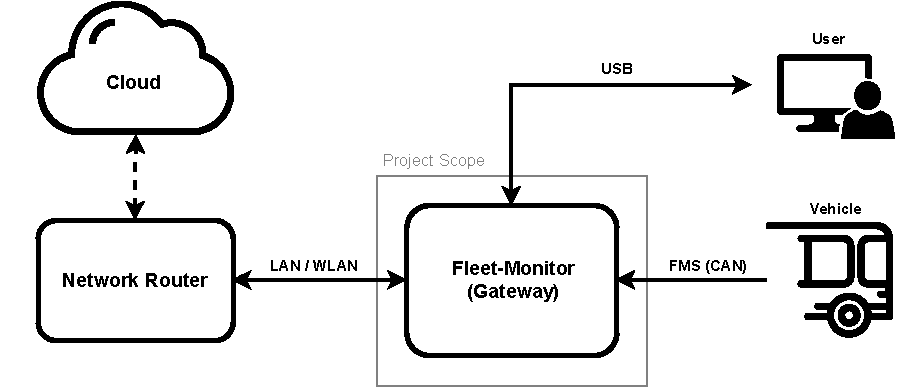
\includegraphics[width=\textwidth]{images/System_Overview}
	\vspace{-0.3cm}
	\caption{System Overview}
	\label{fig:system-overview}
\end{figure}

\section{Open Source}
From the beginning, it was decided that everything about the project would be released under an open source license. Both of us are huge supporters of open source and believe it will be the future of engineering. Building upon existing libraries and code under open source licences, allows us to accelerate the design process. Sometimes open source is considered an act of charity, but in our case, the benefits of using it outweigh any closed source processes. All documents and files of the project can be found on our GitHub page. A short description of all the repositories can be found in the Appendix \ref{Data Archive}.
